% Authors: Emily Gosti, Yannan Tuo, Sukrit Arora, Lydia Lee
% Emails: egosti@berkeley.edu, ytuo@berkeley.edu, lydia.lee@berkeley
\qns{Gram-Schmidt Practice}

\meta{
    Prereqs: Knowledge of bases}

\ans{
    Description: Describe the Gram-Schmidt process and what it does, and how to perform it. The objective of the Gram-Schmidt process is to take a set of linearly independent vectors that are not necessarily orthogonal, and create a set of vectors that span the same space and are orthogonal and of unit length. The motivation behind this is that it is often easier to work with vectors that are orthogonal and of unit length.}

\begin{enumerate}
\qitem\label{def_orthonormal}{
    What does it mean for a set of vectors to be orthonormal?}
    
\meta{
    Some linear algebra textbooks use ``orthogonal'' to describe orthonormal sets.}

\ans{
    Orthonormal is a portmanteau of ``orthogonal'' and ``normal;'' a set of vectors is orthonormal if (and only if)
    \begin{itemize}
        \item all vectors are mutually orthogonal i.e. the angle between different vectors is 90$^\circ$) and
        \item each vector is unit length
    \end{itemize}
    The set of $N$ vectors $\{\vec{v_1}, \cdots, \vec{v_N}\}$ is orthonormal if (and only if, by definition)
    $$v_i^Tv_j = \begin{cases}
                    1 &, i=j\\
                    0 &, i\neq j
                \end{cases}$$}

\empt{\vspace{1.5cm}}

\qitem\label{inversion_orthonormal}{
    In standard least squares problems, we have to invert $A^TA$. However, inversions are computationally intensive (not to mention a pain to calculate by hand), and ideally we'd avoid them as much as possible; suppose $A$ is an orthonormal matrix. Does this make solving a least squares problem easier?}

\ans{
    Yes. If $A$ is orthonormal, then $A^TA = I$:
    \begin{align*}
        A^TA &= \begin{bmatrix}
            \horzbar & \vec{a_1}^T & \horzbar\\
            & \vdots &\\
            \horzbar & \vec{a_n}^T & \horzbar\\
        \end{bmatrix}
        \begin{bmatrix}
            \vertbar & & \vertbar\\
            \vec{a_1} & \cdots & \vec{a_n}\\
            \vertbar & & \vertbar\\
        \end{bmatrix}\\
            &= \begin{bmatrix}
                    \vec{a_1}^T\vec{a_1} & \cdots & \vec{a_1}^T\vec{a_n}\\
                    \vdots & \ddots & \vdots\\
                    \vec{a_n}^T\vec{a_1} & \cdots & \vec{a_n}^T\vec{a_n}
                \end{bmatrix}\\
            &= I_n
    \end{align*}
    and the least squares solution $(A^TA)^{-1}A^T\vec{b}$ becomes a simple projection: $A^T \vec{b}$. This saves us a lot computationally, since computing an inverse is fairly intensive.}

\empt{\vspace{1.5cm}}

\qitem\label{span_requirement}{
    Suppose we replace $A$ with an orthonormal matrix $M$. What must be true of this matrix in order for it to give us the same least squares result?}

\ans{
    $M$'s columns must span the same space as $A$, because least squares is equivalent to projecting $\vec{b}$ onto the span (column space) of $A$.}

\qitem\label{span_equivalence}{
    Explain why span($\{\vec{v_1}$, $\vec{v_2}\}$) is equivalent to span($\{\vec{v_1}$, $\vec{v_2} - \alpha\vec{v_1}\}, \alpha \in \mathbb{R}$).}

\meta{
    The idea is to give intuition as to why Gram-Schmidt gives us a set of vectors that spans the same space.}

\ans{
    Showing that two sets $S_1$ and $S_2$ are equal has two parts: $S_1 \subseteq S_2$ \textbf{and} $S_2 \subseteq S_1$. Both of these must be shown to prove equivalence!

    The span of $\{\vec{v_1}$, $\vec{v_2}\}$ is all linear combinations of $\vec{v_1}$ and $\vec{v_2}$:
    $$\left\{\beta_1 \vec{v_1} + \beta_2 \vec{v_2} \,\forall\, \beta_1, \beta_2\in\mathbb{R}\right\}$$
    Writing out span($\vec{v_1}$, $\vec{v_2}-\alpha \vec{v_1}$) and rearranging it a bit:
    \begin{align*}
        \{\beta_3\vec{v_1} + \beta_4(\vec{v_2}-\alpha)\vec{v_1})\,&\forall\, \beta_3, \beta_4\in\mathbb{R}\}\\
        \{(\beta_3-\beta_4\alpha)\vec{v_1}, \beta_4\vec{v_2}\,&\forall\, \beta_3, \beta_4\in\mathbb{R}\}
    \end{align*}
    If we take some arbitrary $\vec{u_1}$ such that $\vec{u_1}\in\text{span}(\vec{v_1}, \vec{v_2})$, it's also in $\text{span}(\vec{v_1}$, $\vec{v_2}-\alpha \vec{v_1})$, so span($\{\vec{v_1}$, $\vec{v_2}\}$) $\in $span($\vec{v_1}$, $\vec{v_2}-\alpha \vec{v_1}$).

    Going the other way, we consider some arbitrary $\vec{u_2}$ such that $\vec{u_2}\in\text{span}(\vec{v_1}, \vec{v_2}-\alpha \vec{v_1})$. Looking at our rearrangement of the second span, we see that $u_2$ must also be in $\text{span}(\vec{v_1}, \vec{v_2})$}

\empt{\vspace{1.5cm}}

\qitem\label{gs_normalize}{
    Consider now you're given a set of vectors $\{\vec{v_1}, \cdots ,\vec{v_N}\}$, and we want to find an orthonormal set of vectors with the same span as the original set. Find a vector $\vec{w_1}$ such that
    \begin{itemize}
        \item span($\vec{w_1}$) = span($\vec{v_1}$)
        \item $\norm{\vec{w_1}}_2 = 1$
    \end{itemize}}

\meta{
    Step 1: Pick an arbitrary vector in the set and normalize it; it needn't be the first vector in the set.}

\ans{
    $$\vec{w_1} = \frac{\vec{v_1}}{\norm{v_1}}$$}

\empt{\vspace{2.5cm}}

\qitem\label{gs_project_indep}{
    Now suppose that your $\vec{w_1}$ from part \ref{gs_normalize} and $\vec{v_2}$ are linearly independent. Remove the $\vec{w_1}$ ``component'' of $\vec{v_2}$ from $\vec{v_2}$. Call the result $\vec{u_2}$ and find $\vec{u_2}^T\vec{w_1}$}

\ans{
    To remove the $\vec{w_1}$ component from $\vec{v_2}$, we subtract the projection of $\vec{v_2}$ on the span of $\vec{w_1}$ from $\vec{v_2}$
    \begin{align*}
        \vec{u_2} &= \vec{v_2} - \text{proj}_{\text{span}(\vec{w_1})}(\vec{v_2})\\
            &= \vec{v_2} - \vec{w_1}(\vec{w_1}^T\vec{w_1})^{-1}\vec{w_1}^T\vec{v_2}\\
            &= \vec{v_2} - \vec{w_1}(\vec{w_1}^T\vec{v_2})
    \end{align*}
    The result is orthogonal to $\vec{w_1}$, so $\vec{u_2}^T\vec{w_1} = 0$.
    }

\meta{
    Consider a simple 2D example:
    \begin{center}
        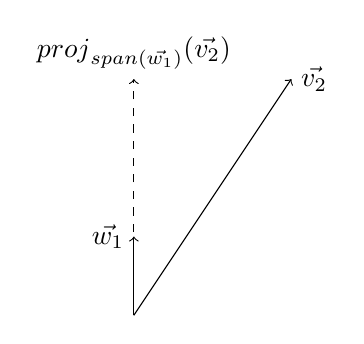
\begin{tikzpicture}
            %% coordinates
            \coordinate (O) at (0,0);
            \coordinate (w1) at (0,1);
            \coordinate (v2) at (2,3);
            \coordinate (proj) at (0,3);

            %% lines
            \draw[->] (O) -- (w1);
            \draw[->] (O) -- (v2);
            \draw[dashed, ->] (O) -- (proj);

            %% point labels
            \node[anchor=east] at (0,1) {$\vec{w_1}$};
            \node[anchor=west] at (2,3) {$\vec{v_2}$};
            \node[anchor=south] at (0,3) {$\text{proj}_{\text{span}(\vec{w_1})}(\vec{v_2})$};
        \end{tikzpicture}
    \end{center}
    Subtracting $\text{proj}_{\text{span}(\vec{w_1})}(\vec{v_2})$ from $\vec{v_2}$ gives us a vector orthogonal to $\vec{w_1}$.}

\empt{\vspace{3cm}}

\qitem\label{gs_project_dep}{
    \textbf{(PRACTICE)} What would happen if $\vec{w_1}$ and $\vec{v_2}$ were linearly dependent and we performed the same operation as in \ref{gs_project_indep}?}
    
\ans{
    We'd get $\vec{u_2} = \vec{0}$. Using the fact that $\norm{w_1} = 1$ to simplify our calculation,
    \begin{align*}
        \vec{v_2} - \vec{w_1}(\vec{w_1}^T\vec{v_2}) &= \vec{w_1}\norm{v_2} - \vec{w_1}\norm{\vec{w_1}}\norm{\vec{v_2}}\\
            &= \vec{w_1}\norm{v_2} - \vec{w_1}\norm{\vec{v_2}}\\
            &= \vec{0}
    \end{align*}}

\meta{
    Graphically,
    \begin{center}
        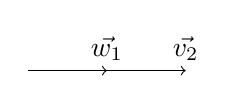
\begin{tikzpicture}
            %% coordinates
            \coordinate (O) at (0,0);
            \coordinate (w1) at (1,0);
            \coordinate (v2) at (2,0);

            %% lines
            \draw[->] (O) -- (w1);
            \draw[->] (O) -- (v2);

            %% point labels
            \node[anchor=south] at (1,0) {$\vec{w_1}$};
            \node[anchor=south] at (2,0) {$\vec{v_2}$};
        \end{tikzpicture}
    \end{center}
    Projecting $\vec{v_2}$ onto $\vec{w_1}$ gives us $\vec{v_2}$, and $\vec{v_2} - \vec{v_2} = \vec{0}$!}

\empt{\vspace{1.5cm}}

\qitem\label{gs_normalize_again}{
    Now go back to assuming $\vec{w_1}$ and $\vec{v_2}$ are linearly independent. Using your answer from parts \ref{gs_project_indep} and \ref{span_equivalence} to find a vector $\vec{w_2}$ such that
    \begin{itemize}
        \item $\vec{w_2}^T\vec{w_1} = 0$
        \item $\norm{\vec{w_2}} = 1$
        \item span($\vec{w_1}, \vec{w_2}$) = span($\vec{v_1}, \vec{v_2}$)
    \end{itemize}}

\meta{
    Step 2: Find the orthonormalized second vector in the new orthonormal set by first calculating the projection of the original second vector onto the orthonormalized first vector, and  second subtracting this value from the original second vector. Finally, normalize the vector.}

\ans{
    Starting with $\vec{v_2}$, we want to remove any component of $\vec{w_1}$ so the resulting vectors are mutually orthogonal and still span the same space as $\left\{\vec{w_1},\vec{v_2}\right\}$.

    Using our work from part \ref{gs_normalize_again}, we get
    $$\vec{u_2} = \vec{v_2} - (\vec{v_2}^T\vec{w_1}){\vec{w_1}}$$
    We know $\vec{u_2}^T\vec{w_1} = 0$ and that span($\vec{w_1}, \vec{u_2}$) is the same as span($\vec{w_1}, \vec{v_2}$), so all we have left to do is ensure that we have a normalized vector
    $$\vec{w_2} = \frac{\vec{u_2}}{\norm{\vec{u_2}}}$$}

\empt{\vspace{1.5cm}}

\qitem{
    For every subsequent vector that we add to our orthonormal set, we want to ensure that it is orthogonal to the rest of the $\vec{w}$'s we've already found. Suppose $\vec{v_3}$ in the original set is linearly independent with respect to $\vec{w_1}$ and $\vec{w_2}$. Derive an expression for the calculating the third vector in the orthonormal set, $\vec{w_3}$.
}

\meta{
    Step 3: For every subsequent vector, repeat the same process, but subtract the projection of the current vector onto every other orthnormalized vector from the current vector. You can also 
}

\ans{
    Let us call the non-normalized, orthogonal vector $\vec{u_3}$.
    \begin{align*}
        \vec{u_3} &= \vec{v_3} - \text{proj}_{\text{span}(\vec{w_2})}(\vec{v_3}) - \text{proj}_{\text{span}(\vec{w_1})}(\vec{v_3})\\
            &= \vec{v_3} - (\vec{v_3}^T\vec{w_2}){\vec{w_2}} - (\vec{v_3}^T\vec{w_1}){\vec{w_1}}
    \end{align*}
    where $(\vec{v_3}^T\vec{w_2}){\vec{w_2}}$ is the projection of the original third vector $\vec{v_3}$ onto the second orthonormal vector $\vec{w_2}$, and $(\vec{v_3}^T\vec{w_1}){\vec{w_1}}$ is the projection of the original third vector onto the first orthonormal vector $\vec{w_1}$ of our new set. Again, we want to normalize the resulting vector, so $$\vec{w_3} = \frac{\vec{u_3}}{\norm{\vec{u_3}}}$$}

\empt{\vspace{3cm}}

\qitem\label{numerical_example}{
    Perform Gram-Schmidt on the following vectors to create an orthonormal basis that spans the same space:
    \[\vec{v_1} = \begin{bmatrix}1\\-1\\1\end{bmatrix}
    \vec{v_2} = \begin{bmatrix}1\\0\\1\end{bmatrix}
    \vec{v_3} = \begin{bmatrix}1\\1\\2\end{bmatrix} \]
}

\ans{
    For the first step, we just take the first vector in the original set, and set it as the first vector in our orthonormal set:
    \[\vec{w_1} = \frac{\vec{v_1}}{\norm{\vec{v_1}}} = \frac{1}{\sqrt{3}}\begin{bmatrix}1\\-1\\1\end{bmatrix} = \begin{bmatrix}\frac{1}{\sqrt{3}}\\-\frac{1}{\sqrt{3}}\\\frac{1}{\sqrt{3}}\end{bmatrix} \]

    Next, let's find $\vec{u_2}$, the un-normalized second vector for our orthonormal set, using $\vec{v_2}$:
    \[\vec{u_2} = \vec{v_2} - (\vec{v_2}^{\top}\vec{w_1})\vec{w_1} = \begin{bmatrix}1\\0\\1\end{bmatrix} - (\begin{bmatrix}1 & 0 & 1\end{bmatrix}\begin{bmatrix}\frac{1}{\sqrt{3}}\\-\frac{1}{\sqrt{3}}\\\frac{1}{\sqrt{3}}\end{bmatrix})\begin{bmatrix}\frac{1}{\sqrt{3}}\\-\frac{1}{\sqrt{3}}\\\frac{1}{\sqrt{3}}\end{bmatrix} = \begin{bmatrix}\frac{1}{3}\\\frac{2}{3}\\\frac{1}{3}\end{bmatrix} \]

    If we want to add this vector to our orthonormal set, we have to normalize it:
    \[\vec{w_2} = \sqrt{\frac{3}{2}}\begin{bmatrix}\frac{1}{3}\\\frac{2}{3}\\\frac{1}{3}\end{bmatrix} = \begin{bmatrix}\frac{\sqrt{6}}{6}\\\frac{\sqrt{6}}{3}\\\frac{\sqrt{6}}{6}\end{bmatrix}
    \]

    Finally, we repeat the same process to find $p_3$ and $w_3$.
    \[\vec{u_3} = \vec{v_3} - (\vec{v_3}^T\vec{w_1})\vec{w_1} - (\vec{v_3}^T\vec{w_2})\vec{w_2} = \begin{bmatrix}1\\1\\2\end{bmatrix} - (\begin{bmatrix}1 & 1 & 2\end{bmatrix}\begin{bmatrix}\frac{1}{3}\\\frac{2}{3}\\\frac{1}{3}\end{bmatrix})\begin{bmatrix}\frac{1}{3}\\\frac{2}{3}\\\frac{1}{3}\end{bmatrix} - (\begin{bmatrix}1 & 1 & 2\end{bmatrix}\begin{bmatrix}\frac{\sqrt{6}}{6}\\\frac{\sqrt{6}}{3}\\\frac{\sqrt{6}}{6}\end{bmatrix})\begin{bmatrix}\frac{\sqrt{6}}{6}\\\frac{\sqrt{6}}{3}\\\frac{\sqrt{6}}{6}\end{bmatrix} = \begin{bmatrix}\frac{-1}{2}\\0\\\frac{1}{2}\end{bmatrix}\]
    \[w_3 = \sqrt{2}\begin{bmatrix}\frac{-1}{2}\\0\\\frac{1}{2}\end{bmatrix} = \begin{bmatrix}\frac{-\sqrt{2}}{2}\\0\\\frac{\sqrt{2}}{2}\end{bmatrix}\]}
\empt{\newpage}
\end{enumerate}